\section{Epidemien - SIR-Modell}
\label{sec:epidemiology-sir-model}

\begin{code}
	\caption{Skript für die Simulation mit einem SIR-Modell}
	\mSourceFile{\srcDir/epidemiologySIRProg.m}
	\label{source:epidemiology-sir-program}
\end{code}

\begin{code}
	\caption{Funktion zur Berechnung des SIR-Modell}
	\mSourceFile{\srcDir/epidemiologySIR.m}
	\label{source:epidemiology-sir}
\end{code}
\ \newpage

\begin{figure}[h]
	\centering
	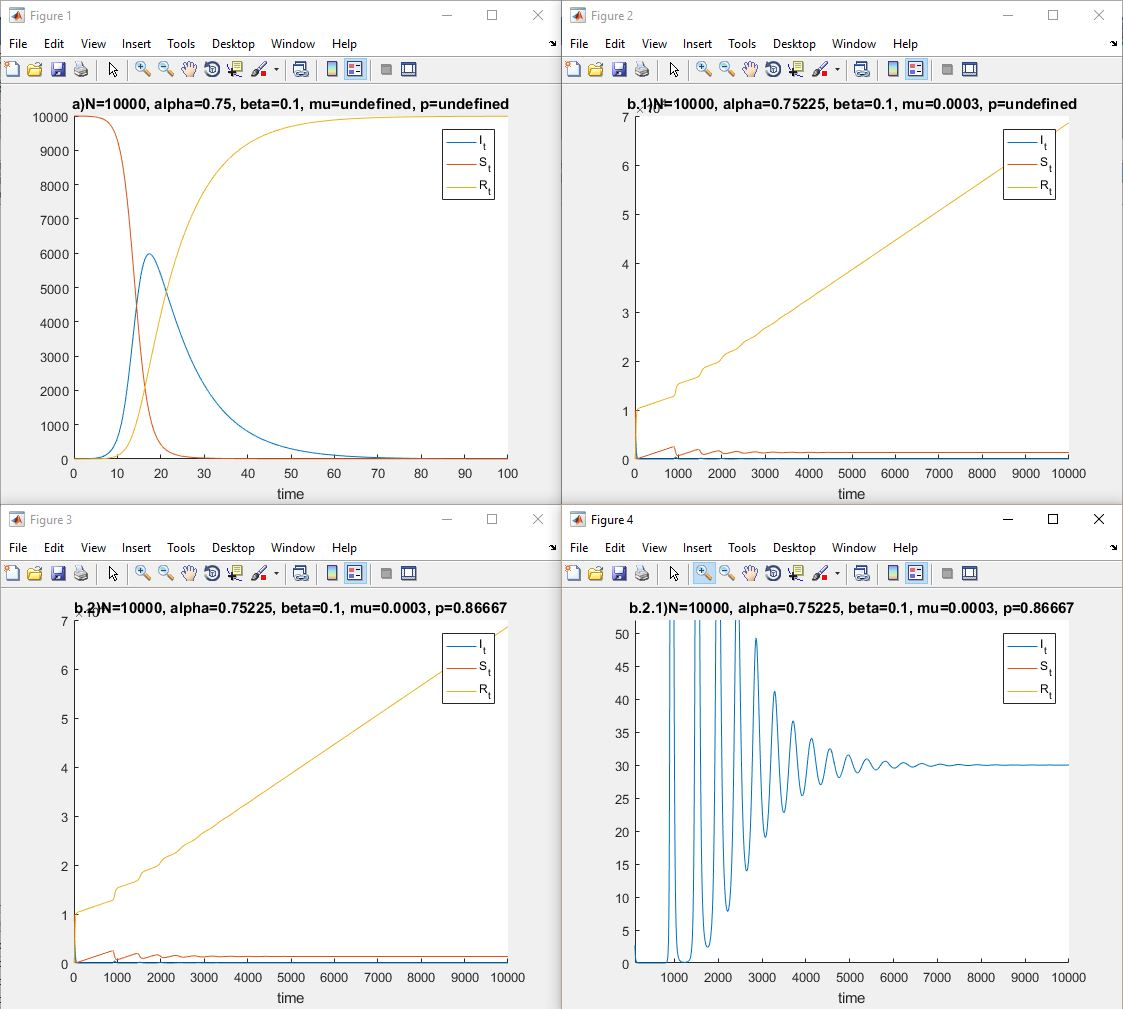
\includegraphics[scale=0.55]{\imageDir/epiomology-sir.JPG}
	\caption{Verlauf der Epidemie mit SIR-Modell}
	\label{test:epidemiology-sir}
\end{figure}
\ \newline
Der erste Ausbruch der Epidemie dauert ca. 60 Tage. Wenn eine Geburtenrate und $p_crit$ miteinbezogen werden, dann sieht man dass sich die Anzahl der infizierten Personen ab ca. 6000 Tagen ungefähr bei 30 Personen einpendelt (Equilibrium).
